\documentclass{ltxdoc}

\usepackage[margin=2.54cm]{geometry}
\usepackage{graphicx}
\usepackage{parskip}
\usepackage{listings}
\usepackage{adjustbox}
\usepackage{soul}
\usepackage{hyperref}
\usepackage{xcolor}
\usepackage{amsmath}
\usepackage{fancyhdr}
\usepackage{titlesec}
\def\sectionbreak{\clearpage}

\pagestyle{fancy}

\expandafter\newif\csname ifuseownpackage\endcsname
\useownpackagetrue

\ifuseownpackage
    \usepackage{highlightlatex}
    \updatehighlight{
    	name = default,
    	add = {
    		\defaultgobble, \colorlet, \includegraphics, \maketitle, \mycommand,
			\tableofcontents, \figref, \color
	    },
		%
    	name = hll,
    	color = orange!90!black,
    	add = {
    		\hll, highlightblock
    	},
		%
    	name = hllOth,
    	color = red!90!black,
    	add = {
    		\useblock, \consumeblock, \updatehighlight, saveblock, \hllconfigure
    	},
		%
    	name = vert,
    	color = red,
    	add = {
    		|
	    }
	}

	\hllconfigure{
		tabsize=4,
		gobbletabs=2
	}
\else
    \let\hll\lstinline
    \lstnewenvironment{highlightblock}[1][]
    {%
        \lstset{#1}%
    }{}%
    \lstset{tabsize=4,escapeinside=~~}
\fi

\newcommand\fhref[2]{%
	\href{#1}{#2}\;\footnote{\,\url{#1}}\,%
}

\newlength\centerlabelledwidth
\newlength\centerlabelledminleft
\def\centerlabelledlabel{}
\setlength\centerlabelledminleft{5em}
\expandafter\newif\csname ifshowcasecenter\endcsname

\makeatletter
\define@key{centerlabelled}{label}{%
	\def\centerlabelledlabel{#1}%
}

\define@key{centerlabelled}{width}{%
	\setlength\centerlabelledwidth{\dimexpr #1\relax}%
}

\define@key{centerlabelled}{frac}{%
	\setlength\centerlabelledwidth{\dimexpr #1\textwidth\relax}%
}

\define@key{centerlabelled}{left}[]{%
	\showcasecenterfalse
}

\define@key{centerlabelled}{center}[]{%
	\showcasecentertrue
}

\define@key{centerlabelled}{minleft}{%
	\setlength\centerlabelledminleft{#1}%
}
\makeatother

\newlength\showcaseleft

\newenvironment{centerlabelled}[1][]{%
	\setlength\centerlabelledwidth{\linewidth}%
	\setkeys{centerlabelled}{#1}%
	\setlength\showcaseleft{\dimexpr(\linewidth-\centerlabelledwidth)/2\relax}%
	\ifshowcasecenter
		\ifdim\centerlabelledminleft>\showcaseleft\relax
			\showcasecenterfalse
		\fi
	\fi
	%
	\unless\ifshowcasecenter
		\setlength\showcaseleft\centerlabelledminleft
		\ifdim\dimexpr\textwidth-\centerlabelledminleft\relax<\centerlabelledwidth\relax
			\setlength\centerlabelledwidth{\dimexpr\linewidth-\centerlabelledminleft\relax}%
		\fi
	\fi
	%
	\par\penalty 10000%
	\hspace{\showcaseleft}%
	\adjustbox{raise=-6pt,lap=-\width-1em}{\setulcolor{red}%
	\expandafter\ul\expandafter{\expandafter\textsc\expandafter{\centerlabelledlabel}}}%
	\begin{minipage}[t]{\centerlabelledwidth}%
	\lstset{framexleftmargin=0.25em}%
}{%
	\end{minipage}\par%
}

\newenvironment{showcase}{%
	\begin{centerlabelled}%
}
{%
	\end{centerlabelled}
}

\makeatletter
\def\option#1{%
	%\item\textbf{#1}%
	\def\term{}%
	\@ifnextchar<{%
		\def\term{\option@i{#1}}%
		\term
	}{%
		\def\term{\option@i{#1}<>}%
		\term
	}%
}

\def\option@i#1<#2>{%
	\@ifnextchar={%
		\option@ii{#1}{#2}%
	}{%
		\option@ii{#1}{#2}={}%
	}%
}

\def\option@ii#1#2=#3{%
	\item\textbf{#1}\texttt{%
		\ifx\relax#2\relax
		\else
			{} = \textlangle #2\textrangle%
		\fi
		,%
		\ifx\relax#3\relax
		\else
			\;[= #3]%
		\fi
	}%
	\par\nobreak
}


\makeatother

\newenvironment{optionlist}{
	\begin{list}{}{
		\itemindent-\leftmargin
		\setlength{\itemsep}{10pt}
	}
%	\let\origitem\item
%	\def\item##1{
%		\origitem\textbf{##1}
%	}
%	\def\option##1{%
%		\origitem\textbf{##1}%
%	}
}{
	\end{list}
}

\def\sectionautorefname{Section}
\def\subsectionautorefname{Subsection}

\begin{document}

\newbox\cmdintitle
\setbox\cmdintitle=\hbox{\hll|highlightlatex|}
\setbox\cmdintitle=\hbox{\adjustbox{height=2.0\height}{\usebox\cmdintitle}}

\title{Package \usebox\cmdintitle{} manual}
\author{
	Vincent Kuhlmann\\
	\texttt{vincent.kuhlmann@hotmail.com}
}


\maketitle
\begin{abstract}
	The \hll|highlightlatex| package provides colored syntax highlighting for \LaTeX{} source code, without aid from
	outside \LaTeX. The aim is to make this accessible enough so people stop falling back to plain verbatim for this.
	For this, it builds further on the generic `listings' package. An example output is	shown in \autoref{fig:demoOutput}\,.
\end{abstract}

\bigskip

\begin{center}
	{\small\textbf{Repository}}

	\url{https://github.com/vkuhlmann/highlight-latex}
\end{center}

\vspace{5\baselineskip}

\begin{figure}[htbp]
	\centering
	\rule{2cm}{1pt}

	\bigskip
	\IfFileExists{demo/demo.pdf}{
		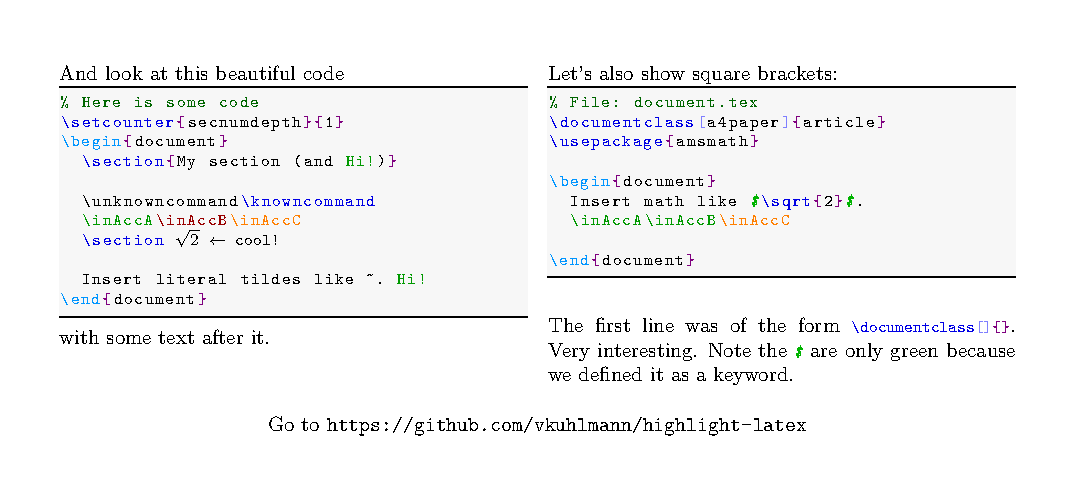
\includegraphics[width=\textwidth,trim=1cm 1cm 1cm 1cm, clip]{demo/demo.pdf}
	}{
		\IfFileExists{demo.pdf}{
			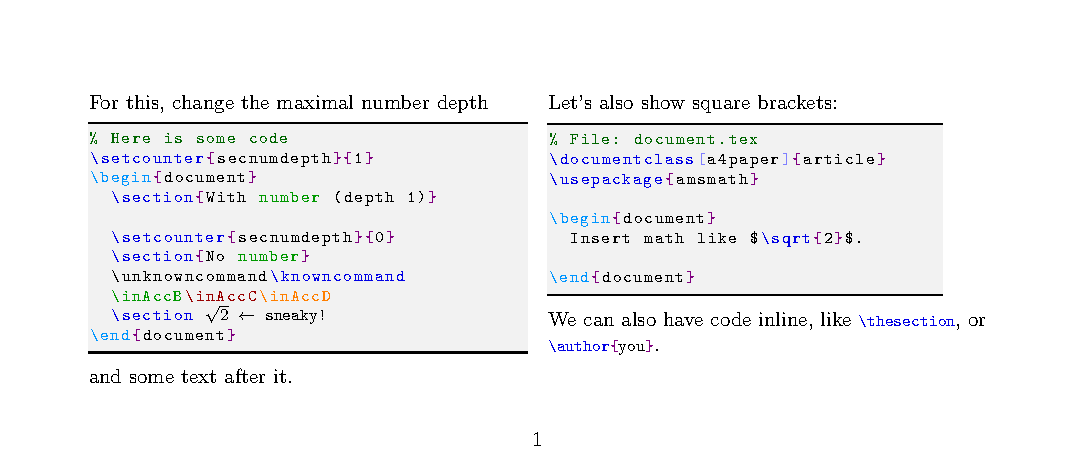
\includegraphics[width=\textwidth,trim=1cm 1cm 1cm 1cm, clip]{demo.pdf}
		}{
			[Generate \texttt{demo.pdf} for an illustration here]
		}
	}
	\caption{Output of `demo.tex'.}\label{fig:demoOutput}
	\bigskip
	\rule{2cm}{1pt}
\end{figure}

\vfil

\pagebreak
\tableofcontents
\pagebreak

\section{Getting started}

Include the package using \hll|\usepackage{highlightlatex}|. If not recognized, refresh your installation's package repository and set it to install \hll|highlightlatex|. There are two ways in which code can be shown.

\subsection{Inline style}

\begin{showcase}[label=example]
	\begin{highlightblock}
		Your file begins with a line of the form \hll~{}~|\documentclass[]{}|. The
		square brackets ...
	\end{highlightblock}
\end{showcase}

\begin{showcase}[label=result]%
	\begingroup
	\adjustbox{cfbox=blue!40!white 2pt 10pt,valign=t,bgcolor=blue!5!white}{%
		\begin{minipage}[t]{\dimexpr\linewidth-24pt\relax}
			Your file begins with a line of the form \hll|\documentclass[]{}|. The
			square brackets ...
		\end{minipage}%
	}%
	\endgroup
\end{showcase}

The first non-space character following \lstinline|\hll| delimits the argument to
this command.

\subsection{Block style}

\begin{showcase}[label=example]
	\begin{highlightblock}
		Your basic document now looks like
		\begin{highlightblock}[gobble=4]
			\documentclass[a4paper]{article}

			\begin{document}
				Hello world!
			\end{document}
		\end{~{}~highlightblock}
	\end{highlightblock}
\end{showcase}

\begin{showcase}[label=result]%
	\begingroup
	\adjustbox{cfbox=blue!40!white 2pt 10pt,valign=t,bgcolor=blue!5!white}{%
		\begin{minipage}[t]{\dimexpr\linewidth-24pt\relax}
			Your basic document now looks like
			\begin{highlightblock}[gobble=16]
				\documentclass[a4paper]{article}

				\begin{document}
					Hello world!
				\end{document}
			\end{highlightblock}
		\end{minipage}%
	}%
	\endgroup
\end{showcase}

\textbf{gobble}. The \hll|gobble| parameter specifies how many characters need to be stripped of the start of each line.
In the example, we had an indentation of four spaces for the literal code. Without the gobble, those spaces would
be shown. See \autoref{sec:globalOther} for setting a global default, and how tabs are interpreted.

% To prevent indentation of our \hll|highlightblock| (here one tab) to be shown as part of the code,
% the \hll|gobble| parameter strips them off. Play around with it until everything looks right. I
% recommend to set this value globally using \hll|\def\defaultgobble{2}|. You can still override it on
% a per-block basis, if necessary.

\textbf{linewidth}. The gray box extends to the width of the page. To set it to only use 60\%, use \hll|linewidth=0.6\linewidth|, or for
a width of 20 characters, set \hll|linewidth=10em|.

%There are situations the block could run out of the page, for example you need to save the block for use in a beamer document (see \autoref{sec:frag}). In that case, the normal full-width of a slide is assumed, but you might want to use it in a slide with multiple columns. Set the \hll|linewidth| on the
%\hll|highlightblock|. This can be a fraction of the total slide width available, \hll|0.6\textwidth|
%is 60\% of the width, or an absolute value, like \hll|10em|, which seems to equal 20 characters.

There are more keys you can provide. Check the
\fhref{https://www.ctan.org/pkg/listings}{\hll|listings| package
	documentation} for options
available to the \hll|lstlisting|-environment and \hll|lstset| command.

\textbf{beamer}. Troubles using beamer? Or troubles with it working at some places, and failing at others? Check \autoref{sec:frag}.

\newbox\uphbox
\setbox\uphbox=\hbox{\hll|\updatehighlight|}
\setbox\uphbox=\hbox{\adjustbox{height=1.4\height}{\usebox\uphbox}}

\section[Macro \textbackslash updatehighlight]{\ignorespaces
  Macro \texorpdfstring{\usebox\uphbox}{\textbackslash updatehighlight}}

\subsection{Examples}

\subsubsection{Adding a command to a highlighting rule}

By default, only some LaTeX commands will be highlighted in blue. If there are others you need, like
\hll|\tableofcontents| and \hll|\figref|, update the highlighting rules:
\begin{showcase}[label=example]
	\begin{highlightblock}
		\updatehighlight{
			name = default,
			add = {
				\tableofcontents, \figref
			}
		}
	\end{highlightblock}
\end{showcase}

The change will only affect code after it. I recommend issuing \hll|updatehighlight| in your
preamble (before the \hll|\begin{document}|). In some situations you might want to change things
mid-document. That's possible too.

\subsubsection{Coloring a command differently}

As shown in \hll|demo.tex|, you can put any command or keyword you want to highlight in a different
color. You do this with
\begin{showcase}[label=example]
	\begin{highlightblock}
		\updatehighlight{
			% The name allows you to modify the style later.
			name = spotlight,
			color = orange,
			add = {
				\tableofcontents
			}
		}
	\end{highlightblock}
\end{showcase}

You can use the \hll|xcolor| syntax for describing colors as well. If you find the orange too
bright, you can replace it with \hll|orange!90!black|: 90\% orange, remaining is black. For more
information on color definitions and name, refer to
\fhref{https://en.wikibooks.org/wiki/LaTeX/Colors}{LaTeX/Colors on Wikibooks}.


\subsection{Specification}

%\begin{showcase}[label=use]
%	\begin{highlightblock}
%		\updatehighlight{
%			option1 = value1,
%			option2 = value2,
%			option3,
%			option4 = value4
%		}
%	\end{highlightblock}
%\end{showcase}

The argument to \hll|\updatehighlight| is a key-value list. Keys are processed in order
and can appear multiple times. If a value contains special characters, like a `=' or `,',
enclose the value with braces. If you want to create some space in your code, don't use
a blank line, they are interpreted by \LaTeX{} as a paragraph end. You can use an empty
line with only a percent sign (\hll|%|) instead.
The processing is done using the package {\setulcolor{red}\ul{xkeyval}}.

You can merge any two \hll|\updatehighlight| in one. No need to close and reopen
\hll|\updatehighlight| for each highlighting rule.

\begin{optionlist}
	\option{name}<characters>

	Sets the named rule to be modified. If a rule with the name does not exist, a new rule will be created.

	There are two default named rules. The first one is \hll|default|, which includes a bunch of basic commands, and has by default
	a dark blue color. The second one is \hll|structure|, which consists of \hll|\begin| and \hll|\end| and prints
	them in light blue.


	\option{classoffset}<integer>

	Sets the \hll|listings| classoffset manually. Try to avoid this. Use \textbf{name} to refer to
	existing rules instead.


	\option{add}<list>

	Adds a command (\hll|\mycommand|) or keyword (\hll|Hi!|) to the current rule. The value can
	contain multiple commands and keywords by seperating them with comma's. The value needs to
	be surrounded with braces.


	\option{remove}<list>

	Removes a commands or keywords from the current rule. The value can
	contain multiple commands and keywords by seperating them with comma's. The value needs to
	be surrounded with braces.


	\option{clear}

	Removes all commands and keywords from the current rule.
	\begin{showcase}[label=example]
		\begin{highlightblock}[gobble=12]
			\updatehighlight{
				name = default,
				clear
			}
		\end{highlightblock}
	\end{showcase}

	\option{color}<color>

	Specifies the current rule's style to color text in the given color. This can also be done using
	the \textbf{style} option, for example \hll|color=red| is equivalent to
	\hll|style=\color{red}|.

	\option{style}<\textrm{\LaTeX{}} code>

	Specifies the current rule's style. A rule can have only one style. If
	you specify a style after \hll|add| or \hll|remove|, this starts a new (unnamed)
	rule. In practice, the only style which will probably work for you is just a
	color. For that, using the `color' key is just a bit easier and neater. But
	hey, you have the option to set whatever style you want. :)

\end{optionlist}

\section{Global settings}

Global parameters can either be set as package option, or through invocation of the
\hll|\hllconfigure|-command.
\begin{showcase}[label=defaults]
	\begin{highlightblock}
		\hllconfigure{
			frame=lines,
			tabsize=4,
			gobble=0,
			backgroundcolor=gray!6!white,
			bracecolor=red!50!blue,
			bracketcolor=blue!50!white,
			commentcolor=green!40!black,
			alsoletter={$@_!|?$},
			mathdollar={
				inner,
				color={green!40!black},
				outer,
				style={\itshape\color{green!70!black}},
				outer%, inner, innerplain, off
			}
		}
	\end{highlightblock}
\end{showcase}

%There are some global parameters involved in the appearance:
%\begin{showcase}[label=overview]
%	\begin{highlightblock}[gobble=8]
%		\colorlet{curlyBrackets}{red!50!blue}
%		\colorlet{squareBrackets}{blue!50!white}
%		\colorlet{codeBackground}{gray!10!white}
%		\colorlet{comment}{green!40!black}
%		\def\defaultgobble{0}
%	\end{highlightblock}
%\end{showcase}

%The package options and \hll|\hllconfigure| take a comma-separated list of key-value pairs.

% The \hll|\hllconfigure| command and package options take a comma-separated list of key-value pairs.
% Each key represents an option. These pairs will be processed in the order they are provided by the user.
% Hence when setting a value multiple times, the last value passed is decisive. However, options can
% involve more than simply setting a value. The exact behavior is described in the specification
% below. The key-value scheme is processed by the package {\setulcolor{red}\ul{xkeyval}}.


The argument to \hll|\hllconfigure| and the value of the package options is a key-value list.
Keys are processed in order
and can appear multiple times. If a value contains special characters, like a `=' or `,',
enclose the value with braces. If you want to create some space in your code, don't use
a blank line, they are interpreted by \LaTeX{} as a paragraph end. You can use an empty
line with only a percent sign (\hll|%|) instead.
The processing is done using the package {\setulcolor{red}\ul{xkeyval}}.

%\begin{showcase}[label=note]
%	\begin{highlightblock}
%		~The key-value scheme is processed by the package {\setulcolor{red}\ul{xkeyval}}.~
%	\end{highlightblock}
%\end{showcase}

%Each line can be set independent of each other, and each shows its default
%value.
%
%There are package options you can use as well:

%The value marked `default' is a value to be set when only the key is specified without being assigned a value. The options available are specified in the following subsections.

The options available are specified in the following subsections.

\subsection{Block appearance}

\begin{optionlist}

\option{frame}<choice>={lines}

	Specifies the frame you want around code blocks. My
	favorites are \hll|lines| and \hll|none|. Check the
	\fhref{https://www.ctan.org/pkg/listings}{listings package documentation} for all
	possibilities.

	The square brackets in the syntax definition above mean you
	can specify `\hll|frame,|' and that this is equivalent to `\hll|frame=lines,|'.

\option{noframe}

	Equivalent to \hll|frame=none|.

\option{debugframe}

	Shows a colored frame around boxes loaded using the \hll|saveblock|+\hll|\useblock| scheme. This can be useful for debugging unexpected offsets. Not for production use.

\option{backgroundcolor}<color>

	Sets the background color of code blocks.

\end{optionlist}

\subsection{General appearance}

\begin{optionlist}
\option{mathdollar}<key-value list>={on}

	Configures styling of code between dollar signs.

	The command takes a key-value list. The allowed keys are
	\begin{optionlist}
		\option{on}
		Enables mathdollar styling.
		\option{off}
		Disables mathdollar styling.

		\option{style}<\textrm{\LaTeX} code>
		Sets style.

		\option{color}<color>
		Sets style to color text with this color. Hence \hll|color=XXX| is equivalent to \hll|style=\color{XXX}|.

		\option{cumulative}<boolean>={true}
		Applies normal coloring rules on top of the style provided.
	\end{optionlist}

	By default, \textbf{mathdollar} is off and has default color \hll|green!40!black| and cumulative enabled. Each invocation of the \textbf{mathdollar} key is implicitly preceded with the option \hll|on|.

\option{bracecolor}<color>

	Sets the color for displaying curly braces (\hll|{| and \hll|}|).

\option{bracketcolor}<color>

	Sets the color for displaying square brackets (\hll|[| and \hll|]|).

\option{commentcolor}<color>

	Sets the color for displaying comments, that is a percent sign (\hll|%|)
	and the text following it.

\end{optionlist}

\subsection{Other}\label{sec:globalOther}

\begin{optionlist}
\option{styleanywhere}

	Overrides the default behavior that \hll|style| starts a new highlighting rule after commands like \hll|add| and \hll|remove|.

\option{tabsize}<integer>

	Sets the amount of space characters a tab character is converted to, when no non-tab character has preceded on the line. Behavior of tab characters is left undefined by this package if a non-tab character has preceded on the line.

\option{gobble}<integer>

	Sets the default amount of characters that will be stripped of code lines within a code block. This is useful to combat indentation used for structuring your \hll|.tex| file to show up in the code block.

\option{gobbletabs}<integer>

	Sets the gobble in amount of \textbf{tabsize}'s. The amount of \textbf{tabsize}'s is evaluated at the start of each code block. The result of \hll|tabsize=4,gobbletabs=2| is equivalent to \hll|gobble=8|. However, when you indent with tabs, this option allows you to quickly change the \textbf{tabsize} without having to update \textbf{gobble} everywhere.

\option{alsoletter}<characters>

	Specifies the character list of special characters to be treated like `letter'. This makes them usable in highlighting rules. However, beware using special characters can conflict with other typesetting routines. Setting this option overrides the previous value.

\end{optionlist}

\section{Fragility}
\label{sec:frag}

\subsection{Introduction}

When passing command arguments around, or storing environment content, \LaTeX{} interprets all
characters. This includes seeing \hll|\maketitle| in \hll!\hll|\maketitle|! as a real command. To
prevent this behavior, everything from \hll|\verb|, \iffalse|\fi to the \hll|verbatim|-environment,
to the \hll|listings| package (which this package depends on) temporarily changes the interpretation
of characters that are still to be read. The blackslash before maketitle in \hll!\hll|\maketitle|!
will be read as `just text' (a \textit{letter} technically).

This reliance on interpretation being done at the last moment is called `fragility'. When content
gets interpreted early, like the \hll|frame|-environment in \hll|beamer| does, this fragility is
broken. A \hll|frame|-environment allows a \hll|fragile| option to be set, which probably solves this,
but I would avoid this. In situations where fragility is broken, you need to either \emph{escape} the
displayed code, or \emph{pre-processing} the displayed code outside a fragile breaking situation.

\subsection{Escaping}

Escaping is done by preceding certain special characters with a backslash. For example,
\hll!\hll|\documentclass[]{}|! becomes \hll!\hll|\\!\hll!documentclass[]\{\}|!.

\subsection{Pre-processing}

For large code blocks, escaping is undesirable. Therefore we pre-process the code when we
have fragility preserved, and load the result in our fragile breaking situation. The storing
is done through the \hll|saveblock|-environment. This environment takes a name under which
the result will be stored. A name can be re-used and will silently overwrite any existing save.

\leavevmode
\begin{showcase}[label=example]
	\begin{highlightblock}
		\begin{saveblock}{basicfigure}
			\begin{highlightblock}[linewidth=0.6\textwidth]
				\begin{figure}
					\includegraphics
					[width=0.9\linewidth]
					{myPlot.pdf}

					\caption{My plot}
					\label{fig:myplot}
				\end{figure}
			\end{highlightblock~{}~}
		\end{saveblock}
	\end{highlightblock}
\end{showcase}

To load the result, use the \hll|\useblock| or \hll|\consumeblock| command
with the save name provided as argument. For the example, these are \hll|\useblock{basicfigure}|
and \hll|\consumeblock{basicfigure}| respectively.

The \hll|\consumeblock| variant
deletes the result from memory after use. This is useful if you have many different save names
occupied. Not deleting them keeps them loaded till the PDF has fully generated. Note \hll|\consumeblock| can
result in unexpected behavior, for example animations in a beamer frame
might need the code line to be executed multiple times. Use \hll|\useblock| when you can't
guarantee the last use of a block.

There is a separate demo for fragile breaking situations. You can find it as
\hll|deamerdemo.tex|.

\section{Adding extra space}

\def\sectionbreak{}

By default, \hll|highlightlatex| follows an approach where it minimizes spacing. This gives you full
control over how tight or spacious your document looks. Just use commands like \hll|\medskip| to add
extra spacing. The package doesn't currently include an option to do it everywhere automatically.

\section{License \& Credits}

The package is available under MIT License. See \textsc{license}.txt.

Thanks for minor fixes:

gemmaro

\rule{5cm}{0.4pt}

For any bug, feature request, unclarity, or whatever else related to this package, you're welcome to
open an issue or pull-request. Issues can be opened on

\begin{showcase}[label=url]
	\begin{highlightblock}[gobble=8]
		~\url{https://github.com/vkuhlmann/highlight-latex/issues}~
	\end{highlightblock}
\end{showcase}

Thanks for contributing!

\end{document}
